\section{Introduction}

\textcolor{red}{Note for later: One of the key patterns I found in the interviews was
that, although many interviewees were empathetic to justice-related efforts and 
initiatives, those initiatives were delegated to a dedicated person or department
within governing institutions. This suggests there is more work to be done 
integrating energy justice and energy modeling/policy-making}

Earlier chapters introduced a novel modeling tool, \ac{osier}, which sought to
fill a gap in the literature and available modeling tools by developing a
flexible multi-objective optimization framework that allows users to incorporate
concepts of justice, the ``human dimension'' \cite{pfenninger_energy_2014}. This
is possible because \ac{osier} enables users to optimize any quantifiable
objective which encourages modelers to seek input from the communities they
model for their energy system priorities, as suggested by McGookin et al. 2024
\cite{mcgookin_advancing_2024}, thereby elevating the recognition and procedural
aspects of justice described in Chapter \ref{chapter:lit-review}. Additionally,
\ac{osier} transcends scale limitations due to it's flexible design, making it
useful for municipalities as well as larger governing units. This chapter
attempts to validate these assertions by examining how local and state energy
planners use \acp{esom} and the ways in which justice does or does not play a
role in decision-making. To that end, this chapter considers a range of contexts
in the State of Illinois, including three municipalities (Champaign, Urbana, and
Naperville), a university with its own microgrid (\acf{uiuc}), and Illinois
energy organizations (\acf{icc}, \acf{ipa}, \acf{icea}, and the Illinois
\acf{cub}). This chapter also considers the varied perspectives of different
energy planning participants within their respective contexts by interviewing
city planners, a city council member, and various advisory staff. This study
contributes to the existing literature on participatory and distributed energy
planning as well as illustrating a path towards a holistic integration of energy
justice and energy system engineering.

The next section reviews the existing literature on decentralized energy
planning. Section \ref{section:interview-methods} describes the method for
collecting and analyzing interview data using thematic analysis. Section
\ref{section:cases} introduces the different cases considered in this chapter.
\textcolor{red}{Lastly, an analysis and discussion of the interviews.}


\section{Literature Review?}

\textcolor{red}{What are some of the novelties of this study}
\begin{enumerate}
    \item Multiple case study that looks at multiple scales of energy governance
    in the state of Illinois. Other studies that investigated multiple cases
    only looked at the energy policy and decision making at the municipal level
    \cite{johannsen_designing_2021, ben_amer_too_2020}.
    \item Another study asked ``What are the differences between energy model
    improvements as perceived by modellers, and the actual needs of users of
    model results'' \cite{susser_better_2022}?
    \item Considers structural barriers to energy modeling.
    \item Investigates the role concepts of energy justice do (or do not) play
    in energy policy for some places in Illinois.
    \item Evaluates a specific energy modeling tool and features of that tool.
\end{enumerate}

\section{Methodology}
\label{section:interview-methods}

\subsection{Thematic Analysis}
This thesis relies on multiple case studies using interviews with energy
planners and decision makers at local and state levels, extending the method
described by Johannsen et al. 2021 \cite{johannsen_designing_2021}. The
interviewees were chosen to be paradigmatic cases (\textcolor{red}{Is this
really what I mean?}) \cite{flyvbjerg_five_2006}. The interviews were
transcribed with the ``listen and revise method'' using the Whisper
transcription tool \cite{battaglia_listen_2024}. Whisper uses \ac{ai} to
automate the transcription process. Both the data and the \ac{ai} model used to
transcribe the interview audio were hosted locally (i.e., without an internet
connection), eliminating privacy concerns \cite{battaglia_listen_2024}. Figure
\ref{fig:whisper} shows a screenshot of the Whisper interface. The interview
coding step was also performed locally with the \texttt{Taguette} tool
\cite{rampin_taguette_2021}. Figure \ref{fig:taguette} shows a screenshot of the
\texttt{Taguette} software.

\begin{figure}
    \centering
    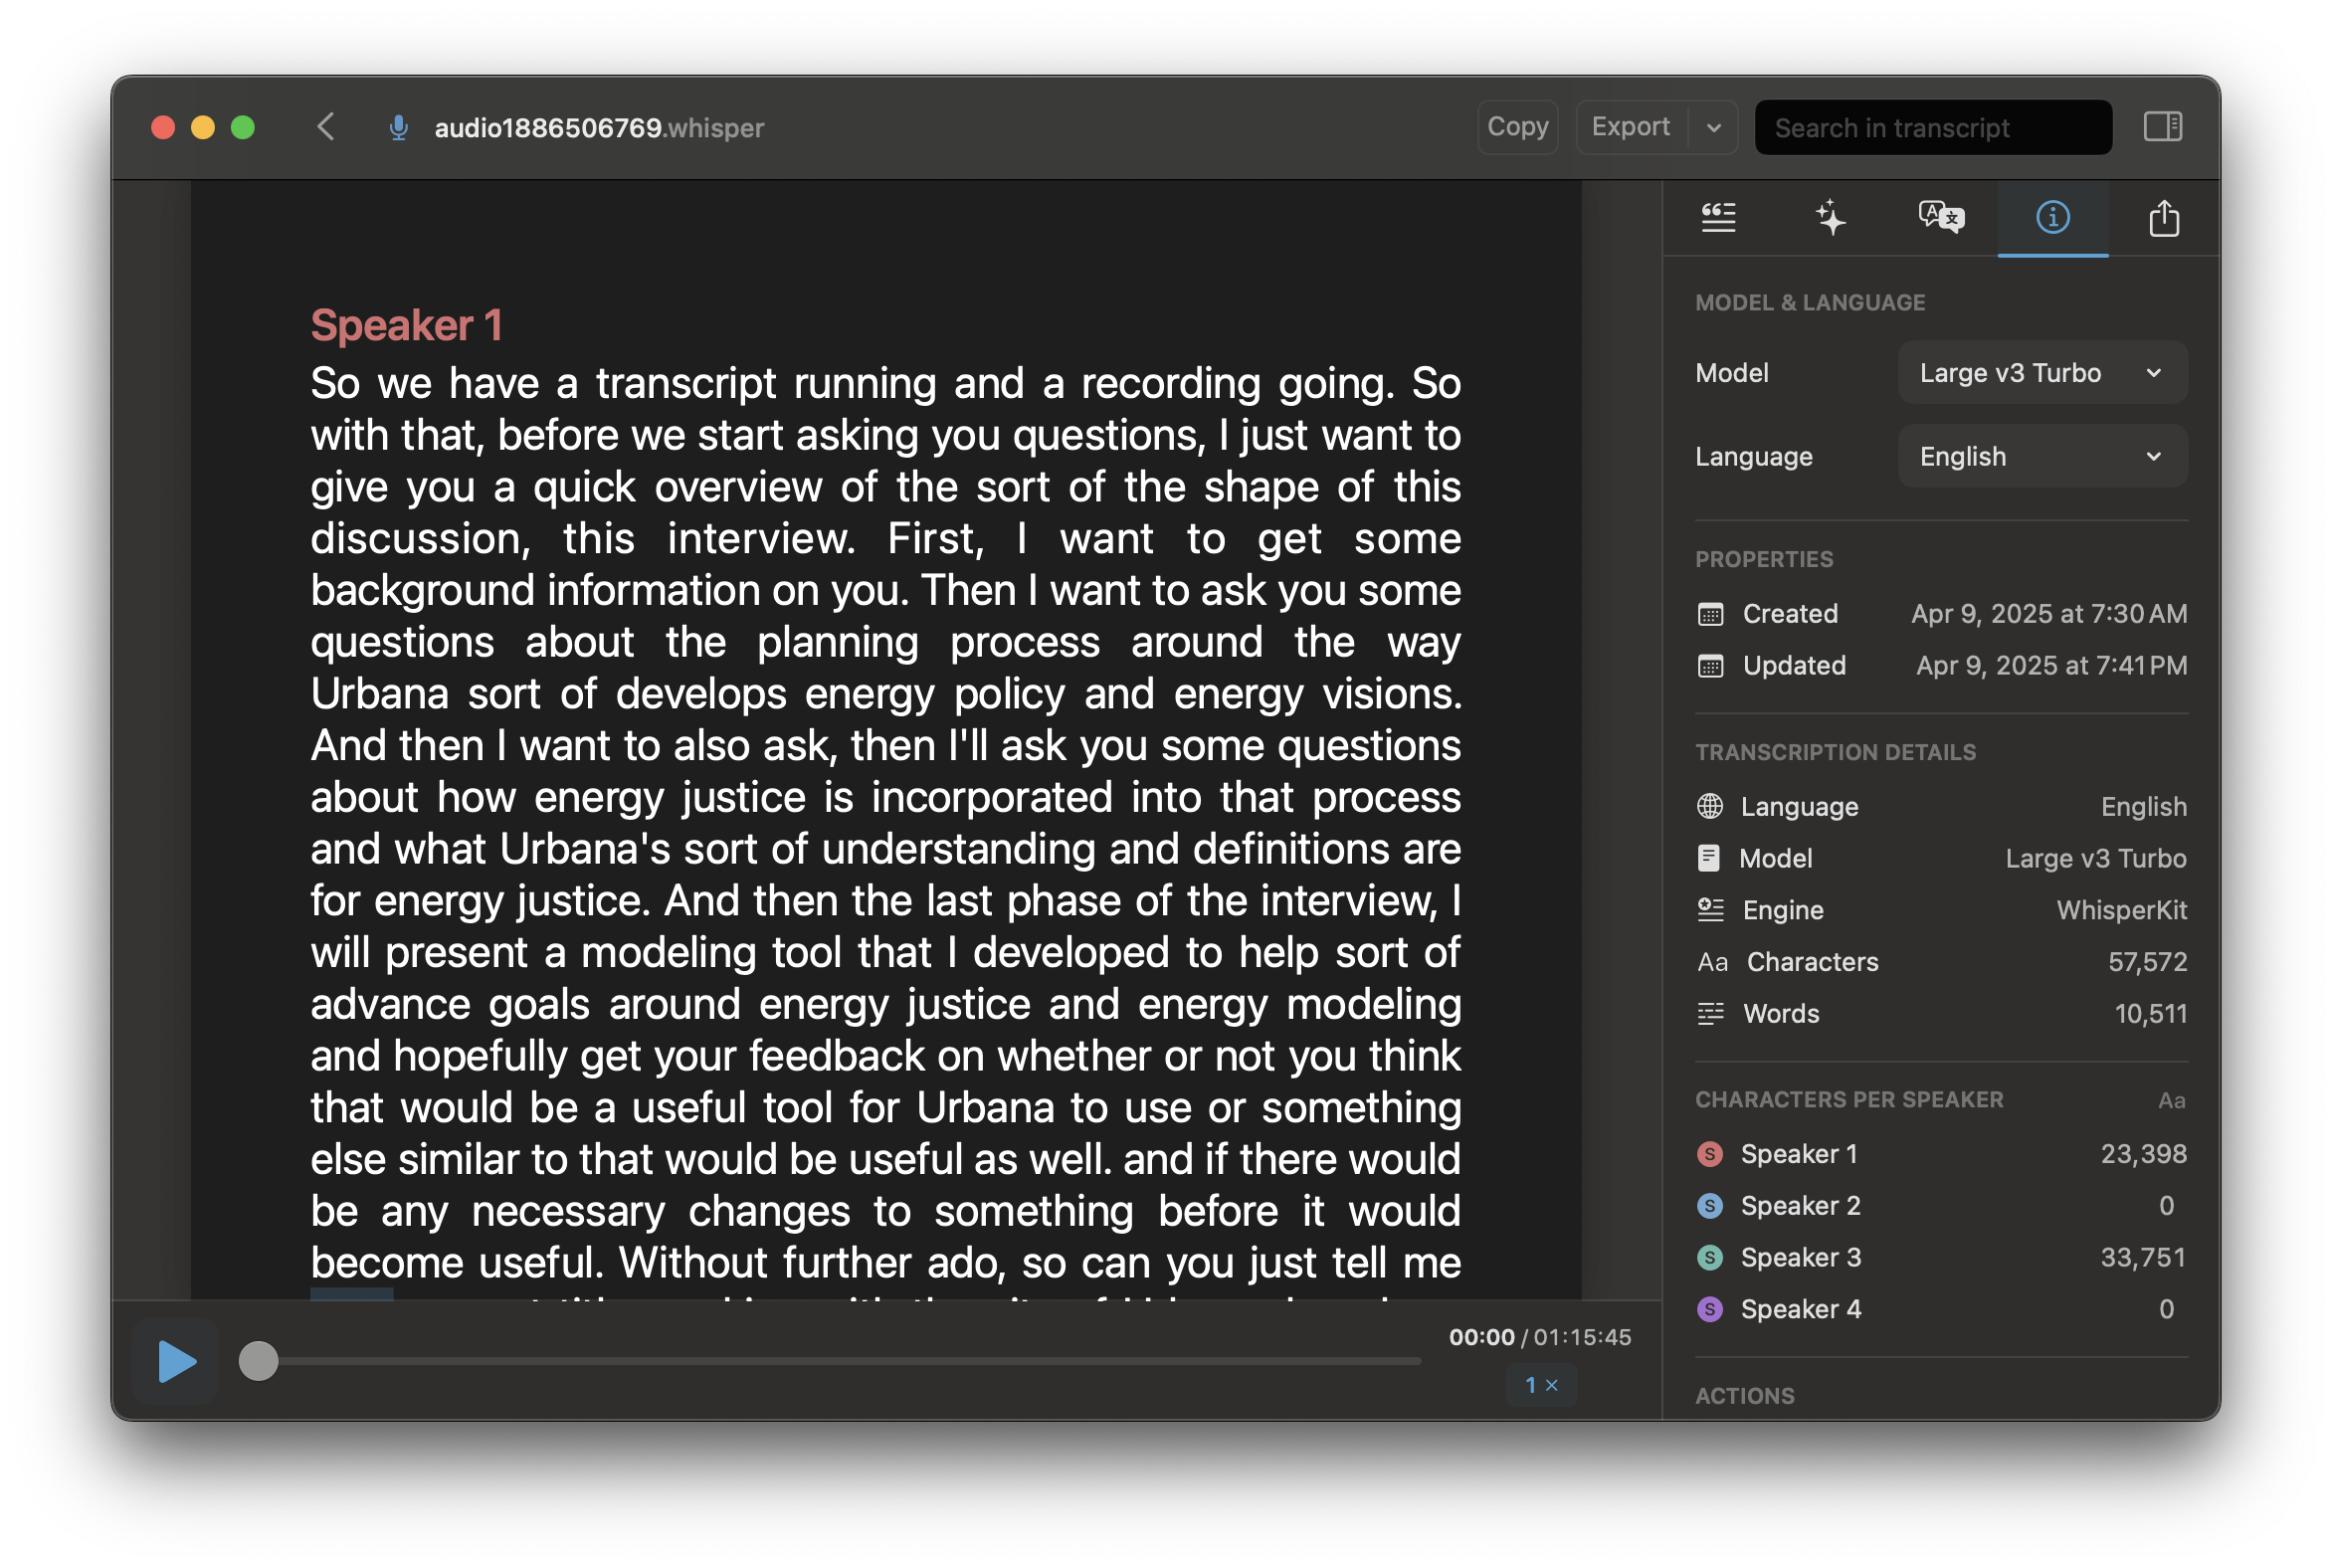
\includegraphics[width=0.6\columnwidth]{figures/07_interview_chapter/whisper-screenshot.png}
    \caption{A screenshot of an interview transcribed with Whisper. To protect
    the privacy of the interviewees, only ``Speaker 1'' is shown. ``Speaker 1''
    is the author of this thesis.}
    \label{fig:whisper}
\end{figure}

\begin{figure}
    \centering
    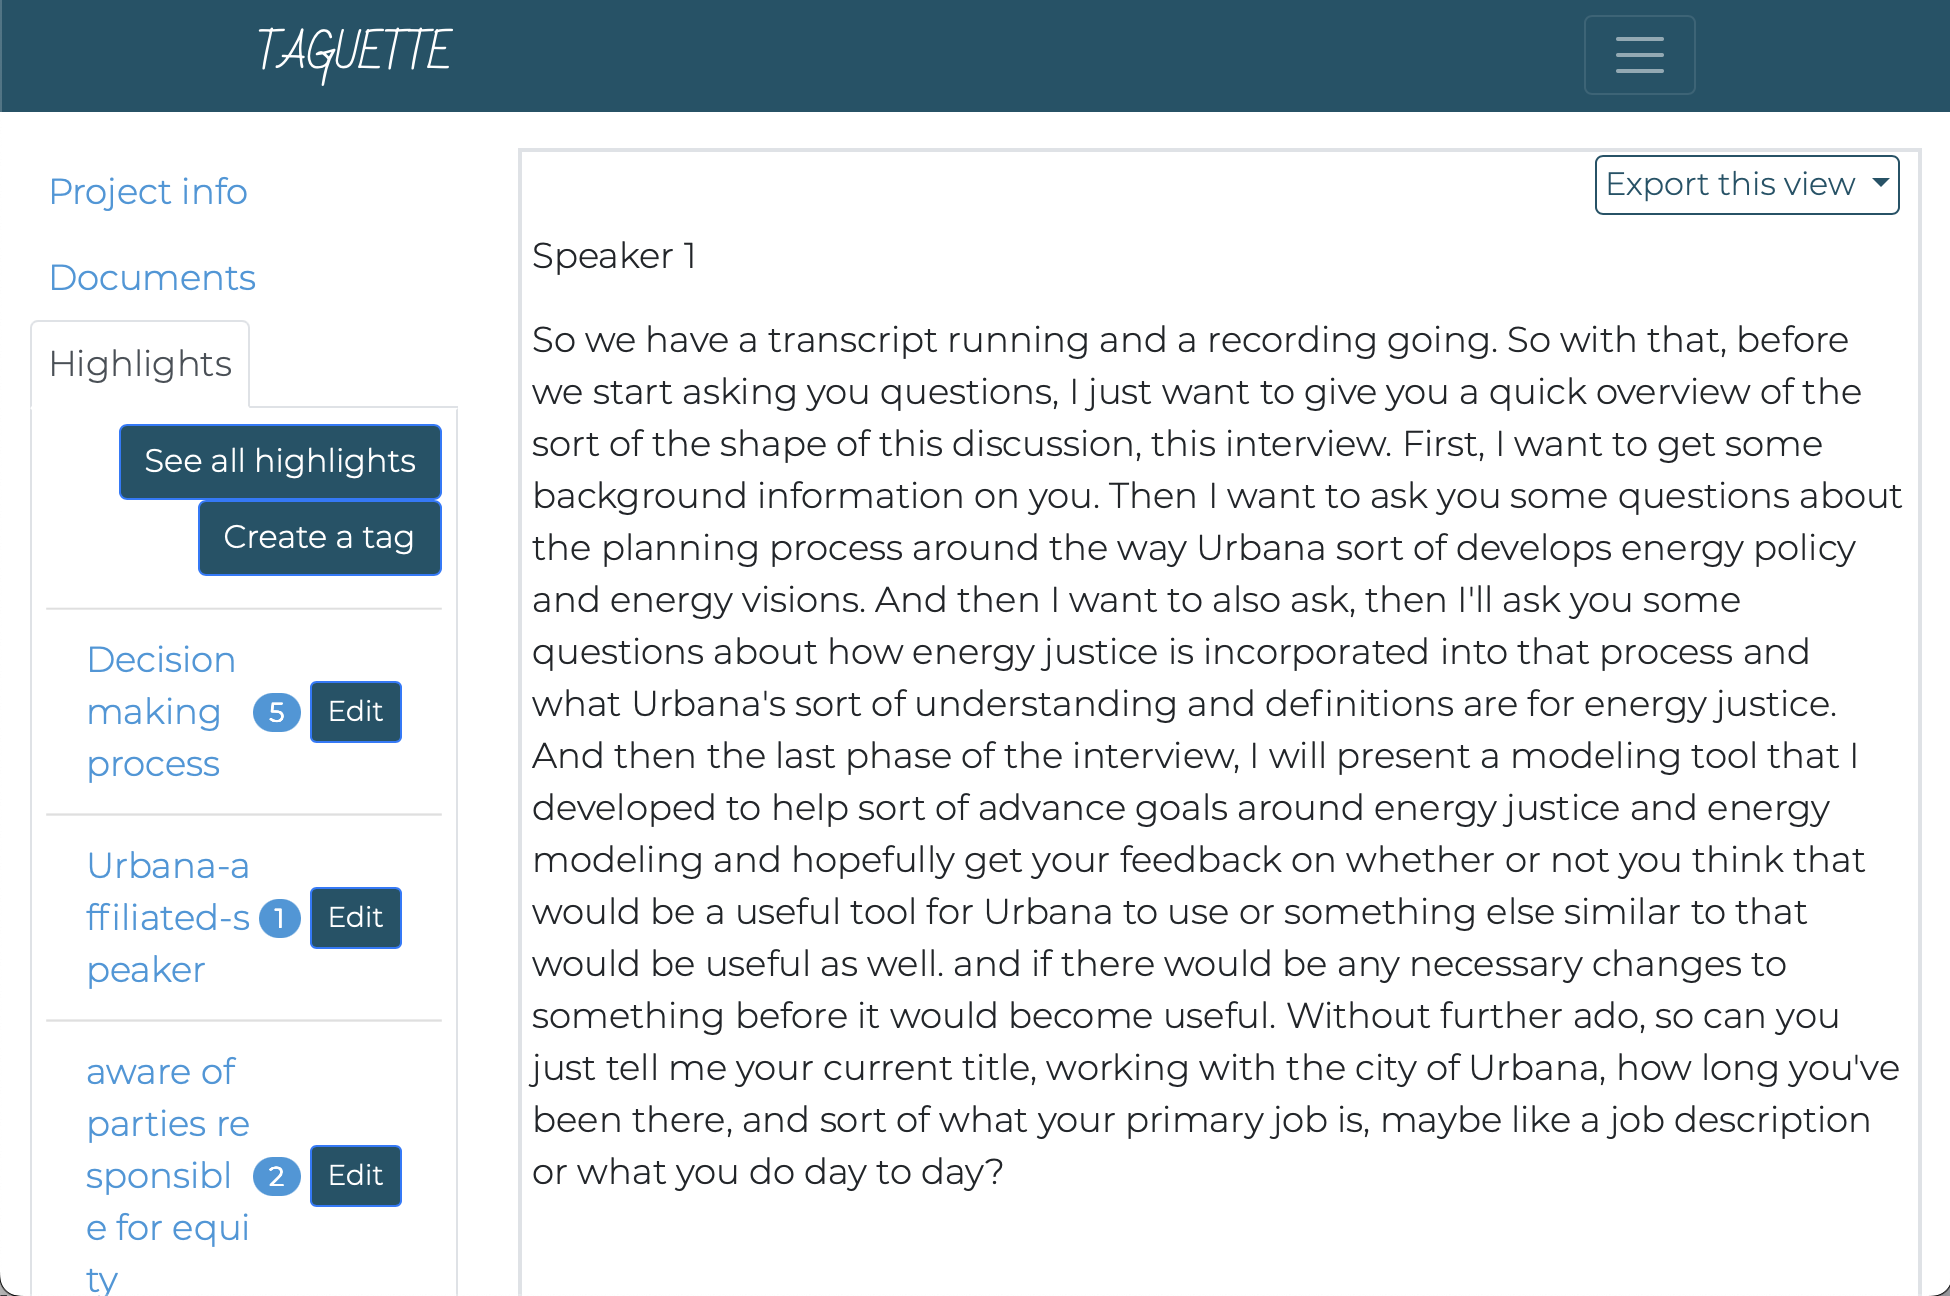
\includegraphics[width=0.6\columnwidth]{figures/07_interview_chapter/taguette-screenshot}
    \caption{A screenshot of the interview transcribed in Figure \ref{fig:whisper}
    loaded into \texttt{Taguette} for initial coding.}
    \label{fig:taguette}
\end{figure}

\subsection{Interview Data Collection}

A total of thirteen interviews were conducted through the second half of 2024
and beginning of 2025 using a semi-structured approach.

\begin{enumerate}
    \item Who did I interview and what organizations were they from?
    \item Why did I choose these interviews?
    \item When were the interviews conducted?
    \item How were the interviews conducted? (i.e., over Zoom)
\end{enumerate}

\section{Case Regions}
\label{section:cases}

Table \ref{tab:demographics} shows the sizes of each planning context by
population.



\subsection{State of Illinois}
Illinois is split between two \acp{rto}, MISO and PJM.

\begin{enumerate}
    \item \ac{icc}
    \item \ac{ipa}
    \item \ac{icea}
    \item Illinois \ac{cub}
\end{enumerate}



\begin{table}
    \centering
    \caption{Summary demographics for the study regions.}
    \label{tab:demographics}
    \begin{tabular}{llll}
        \toprule
        Region & Population & Operating Budget & Median Household Income \\
        & & (millions of \$) &(\$/year) \\
        \midrule
        Illinois
        \cite{united_states_census_bureau_quickfacts_2024-3,sturm_illinois_2024}&
        12,710,158  & 53,419 & 81,702\\
        Naperville
        \cite{united_states_census_bureau_quickfacts_2024-2,munch_annual_2024} &
        150,249  & 641 & 150,937 \\
        Champaign
        \cite{united_states_census_bureau_quickfacts_2024,nees_adopted_2024} &
        89,189 & 210 & 57,544 \\
        Urbana \cite{united_states_census_bureau_quickfacts_2024-1,
        ho_city_2024}& 38,201 & 85 & 45,854 \\
        \ac{uiuc} \cite{data_usa_university_2022,
        university_of_illinois_system_fy_2024} & 59,916 & 3,078 & N/A \\
        \bottomrule
    \end{tabular}
\end{table}

\subsection{Champaign and Urbana, Illinois}
These two contexts are considered together due to their proximity and close
relationship. 

Here are their climate action plans...

\subsection{\acf{uiuc}} 

The \acl{uiuc} (\acs{uiuc} or ``The University''), Illinois' largest
university, straddles the two municipalities of Champaign and Urbana and its
student enrollment rivals the populations of its neighbors. \ac{uiuc} has
uniquely diverse energy system including a wholly owned subsidiary company,
\ac{pei}, that owns and operates energy supply and distribution for the campus
\cite{affiliated_engineers_inc_utilities_2015}. \ac{pei} also enables \ac{uiuc}
to participate in the open electricity market, buying and selling wholesale electricity.
On the supply side, \ac{pei} owns a coal and natural gas cogeneration plant, Abbott Power Plant, which
produces steam and electricity for the campus, as well as a chilled water
storage system. \ac{uiuc} also has \acp{ppa} for wind
\cite{breitweiser_wind_2016} and solar energy \cite{white_solar_2017,
white_solar_2020} along with solar panels on several campus buildings. 
On the distribution side, \ac{pei} operates steam, electric, and
gas distribution for the campus. 

Here is its climate action plan...

\subsection{Naperville, Illinois}
Naperville is interesting because it owns the distribution utility that serves
electricity but does not own any generation.
\begin{enumerate}
    \item \ac{nest}
    \item City of Naperville (Sustainability Department)
\end{enumerate}

\section{Energy Planning in Illinois}

This section answers the following questions
\begin{enumerate}
    \item Where do consumers get their energy from? For example, the open energy
    market, their municipality, municipal electric aggregation, or some default
    supply decided by the state of Illinois.
    \item How do suppliers of electricity, decide what types of generators in
    which to invest? For example, the \ac{imea} procures electricity on behalf
    of their member communities from the open market, and also owns part of the
    Prairie coal plant.
\end{enumerate}



% This chapter addresses my proposal to ``validate'' \ac{osier} by conducting a
% case study of energy planning processes in Champaign-Urbana through interviews
% with decision makers and planners about energy justice, energy modeling, and
% energy planning. As well as introduce interviewees to \ac{osier} itself and
% solicit feedback from them about its potential usefulness and what obstacles
% may interfere with its adoption. 

% Although I originally set out to conduct a limited case study of Chambana, I
% discovered that municipalities in Illinois do not, in general, have the
% decision making authority to make specific choices about their energy supply.
% Thus, I expanded my study to the state level; interviewing people from the
% \ac{ipa} and \ac{icc}. This expanded scope provided evidence for structural
% challenges blocking municipal influence from energy planning processes.
% Further, this evinces a tension among distributive, procedural, and
% recognition justice.

% \section{Progress on developing tools for local use}

% \begin{itemize} \item The literature review chapter indicated that most energy
%     modeling tools and much of the related literature focus on state- or
%     national-scale energy systems. \item The the hyper-local section
%     highlighted some studies that integrated local perspectives with energy
%     modeling. Those papers include \cite{mckenna_combining_2018,
%     johannsen_municipal_2023, fleischhacker_portfolio_2019} \item There have
%     also been studies investigating the development of models for, and use by,
%     city and urban planners. \end{itemize}

% \section{Municipal Levers: How municipalities make choices about their energy
% supply} There are generally four ways municipalities can make choices about
% their energy supply.

% \subsection{\ac{mca}} This is where municipalities participate in electricity
% markets on behalf of their residents. Although this allows municipalities to
% choose an energy supply besides the standard portfolio provided by an electric
% utility, municipalities do not have full control over their energy supply.
% Instead, municipalities negotiate for a few portfolios through a bidding
% process. While they can specify some criteria, such as a percentage of
% renewable energy, the specific generation mix depends on the company that
% developed the portfolio bid. Further, residents are still allowed to opt-out
% of \ac{mca} and elect the standard portfolio provided by their electric
% utility.

% \subsection{Utility ownership} Some municipalities in Illinois, such as
% Naperville, own their own distribution system. This gives a municipality
% greater control over the design of their utility system and allows a
% municipality to make decisions about the tradeoff between cost and resiliency.
% For example, Naperville undergounded most of the electric distribution system
% and new distribution is automatically undergounded. However, this model does
% not award control of electric supply to the municipality, which must procure
% electricity through another entity such as the \acf{imea}.

% \subsection{Municipal-owned generation} In very few cases, a municipality may
% own some of its own generation. \ac{uiuc} owns a coal and natural gas plant, a
% solar array, chilled water storage, and participates in a \ac{ppa} to purchase
% wind power. More commonly, municipalities will lease land cheaply to a solar
% company, for example, and purchase some or all of the rights to that
% electricity through a \ac{ppa}. 

% \subsection{Municipal-owned buildings}